\documentclass[aspectratio=169,11pt]{beamer}
\usetheme[progressbar=frametitle,numbering=fraction,block=fill]{metropolis}
\usepackage[T1]{fontenc}
\usepackage[utf8]{inputenc}
\usepackage[spanish,provide=*]{babel}
\usepackage[scaled=0.95]{helvet}
\usepackage{amsmath,amssymb,bm}
\usepackage{booktabs}
\usepackage{tikz}
\usetikzlibrary{arrows.meta,positioning,calc,fit,backgrounds,shapes.geometric}

\definecolor{azul}{HTML}{2A78D6}
\definecolor{naranja}{HTML}{EB6834}
\definecolor{verde}{HTML}{1BAF7A}
\definecolor{gris}{HTML}{52514E}
\definecolor{fondo}{HTML}{23373B}
\setbeamercolor{alerted text}{fg=naranja}
\setbeamercolor{progress bar}{fg=azul}
\setbeamercolor{frametitle}{bg=fondo}
\setbeamercolor{block title}{bg=azul!15,fg=fondo}
\setbeamercolor{block body}{bg=azul!5}

\tikzset{caja/.style={draw=#1, fill=#1!10, rounded corners=4pt, minimum width=36mm, minimum height=15mm, align=center, font=\small}}

\newcommand{\Rh}{\hat R}
\newcommand{\Sh}{\hat S}
\newcommand{\Pih}{\hat\Pi}
\newcommand{\rstar}{r^{\ast}}
\newcommand{\Pre}{\operatorname{Pre}}

\title{Repetición espaciada sobre grafos de habilidades procedimentales}
\subtitle{Modelo, simulador y primeros resultados}
\author{Gustavo S. de la Rosa}
\institute{Proyecto de maestría --- reunión con el asesor}
\date{Octubre de 2026}

\begin{document}

\maketitle

%---------------------------------------------------------------
\begin{frame}{El problema}
\small
\begin{columns}[T]
\column{0.5\textwidth}
\textbf{Lo que existe}
\begin{itemize}
\item SM-2, FSRS, MEMORIZE (Tabibian 2019): una tarjeta = \alert{una} pieza de conocimiento.
\item Ítems independientes entre sí.
\item Funciona muy bien para \emph{hechos}.
\end{itemize}
\column{0.5\textwidth}
\textbf{Lo que pasa en física}
\begin{itemize}
\item Un problema de tiro parabólico usa vectores, MUA \emph{y} composición de movimientos.
\item Si falla, ¿\alert{qué} falló?
\item Hay un orden: sin MUA no hay tiro parabólico.
\item Demasiados temas nuevos saturan la cola de repasos (Reddy 2016).
\end{itemize}
\end{columns}
\vspace{2mm}
\begin{block}{Pregunta}
¿Cómo usar el modelo de olvido $R(t)=e^{-n\Delta t}$ para planificar la práctica de \emph{habilidades} que dependen unas de otras?
\end{block}
\end{frame}

%---------------------------------------------------------------
\begin{frame}{La idea en una frase}
\centering
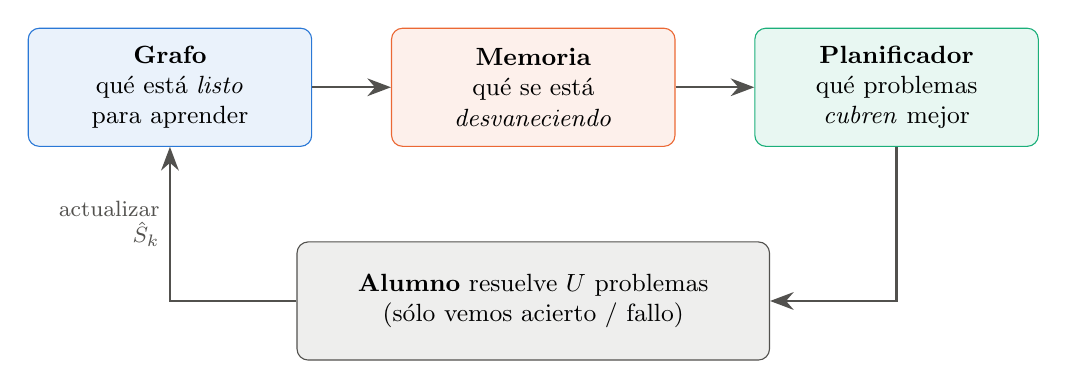
\begin{tikzpicture}[
  fl/.style={-{Stealth[length=3mm]}, thick, gris}
]
\node[caja=azul] (g) {\textbf{Grafo}\\qué está \emph{listo}\\para aprender};
\node[caja=naranja, right=10mm of g] (m) {\textbf{Memoria}\\qué se está\\\emph{desvaneciendo}};
\node[caja=verde, right=10mm of m] (p) {\textbf{Planificador}\\qué problemas\\\emph{cubren} mejor};
\node[caja=gris, below=12mm of m, minimum width=60mm] (a) {\textbf{Alumno} resuelve $U$ problemas\\(sólo vemos acierto / fallo)};
\draw[fl] (g) -- (m);
\draw[fl] (m) -- (p);
\draw[fl] (p) |- (a);
\draw[fl] (a) -| node[pos=0.75, left, font=\footnotesize, align=right]{actualizar\\$\Sh_k$} (g.south);
\end{tikzpicture}
\vspace{5mm}

\small Cada sesión: calcular $\Rh_k$, elegir problemas, observar resultados y actualizar. Los parámetros se estiman con datos de un piloto.
\end{frame}

%---------------------------------------------------------------
\section{El modelo}

\begin{frame}{Pieza 1: grafo y matriz $Q$ fraccional}
\small
\begin{columns}[T]
\column{0.5\textwidth}
\centering
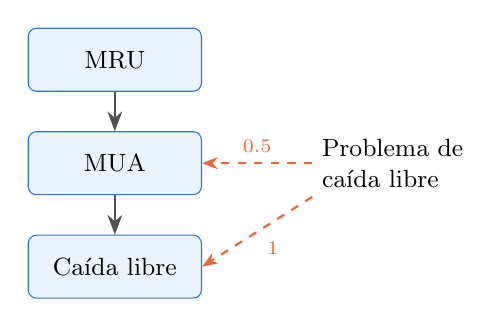
\begin{tikzpicture}[
  nodo/.style={draw=azul, fill=azul!10, rounded corners=3pt, minimum width=22mm, minimum height=8mm, font=\small},
  pre/.style={-{Stealth[length=2.5mm]}, thick, gris}
]
\node[nodo] (mru) {MRU};
\node[nodo, below=5mm of mru] (mua) {MUA};
\node[nodo, below=5mm of mua] (cai) {Caída libre};
\draw[pre] (mru) -- (mua);
\draw[pre] (mua) -- (cai);
\node[right=14mm of mua, font=\small, align=left] (p) {Problema de\\caída libre};
\draw[-{Stealth[length=2mm]}, naranja, dashed, thick] (p.west) -- node[above, font=\scriptsize]{0.5} (mua.east);
\draw[-{Stealth[length=2mm]}, naranja, dashed, thick] (p.south west) -- node[below right, font=\scriptsize]{1} (cai.east);
\end{tikzpicture}
\column{0.5\textwidth}
Un problema del tema $j$ ejercita:
\[
w_{jk}=\begin{cases}1 & k=j\\ 0.5 & k\in\Pre(j)\\ 0 & \text{otro}\end{cases}
\]
\begin{itemize}
\item El tema completo y sus prerrequisitos \alert{a medias}.
\item Crédito implícito: practicar caída libre repasa MUA de paso.
\item Los pesos $w_{jk}$ se pueden estimar con datos.
\end{itemize}
\end{columns}
\end{frame}

%---------------------------------------------------------------
\begin{frame}{Pieza 2: memoria y observación}
\textbf{Memoria} (Tabibian 2019), por habilidad:
\[
\Rh_k(t)=\exp\!\Bigl(-\frac{t-\hat L_k}{\Sh_k}\Bigr)=e^{-\hat n_k\Delta t}
\qquad \Sh_k=\text{estabilidad (días)}
\]
\textbf{Observación}: conjuntiva, con descuido $s$ y adivinanza $g$:
\[
\Pih_j=\prod_{k\in Q(j)}\Rh_k^{\,w_{jk}},\qquad
\Pr(\text{acierto})=(1-s)\,\Pih_j+g\,(1-\Pih_j)
\]
\begin{itemize}
\item Sabe todo $\Rightarrow$ falla sólo por descuido ($s=0.05$).
\item No sabe algo $\Rightarrow$ acierta sólo por adivinanza ($g=0.02$).
\item Esto da una \alert{verosimilitud explícita}, que es lo que permite estimar todo con datos.
\end{itemize}
\end{frame}

%---------------------------------------------------------------
\begin{frame}{Actualización: acierto, salto y culpa}
\begin{columns}[T]
\column{0.5\textwidth}
\textbf{Acierto}: cada componente gana
\[
\Sh_k\leftarrow\Sh_k\,[1+w_{jk}\,G\,(1-\Rh_k)]
\]
\begin{itemize}\small
\item Si $\Rh\approx1$, no gana nada: \alert{efecto de espaciamiento}.
\item La práctica masiva no puede ``dominar'' un tema.
\end{itemize}
\textbf{Salto} (Tabibian): $\Rh_k^+=\Rh_k+w_{jk}(1-\Rh_k)$.

\small Una sola actualización por habilidad por sesión.
\column{0.5\textwidth}
\textbf{Fallo}: culpa bayesiana
\[
b_k=\frac{1-\Rh_k^{\,w_{jk}}}{1-\Pih_j},\qquad \Sh_k\leftarrow\Sh_k(1-\lambda b_k)
\]
\begin{exampleblock}{Ejemplo}
\small $\Rh_{\text{caída}}=0.64$, $\Rh_{\text{MUA}}=0.79$, falla el problema:\\[2pt]
$b_{\text{caída}}=0.84$, \quad $b_{\text{MUA}}=0.26$\\[2pt]
El sistema concluye que el problema está en caída libre, \emph{sin ver} qué pasó.
\end{exampleblock}
\end{columns}
\end{frame}

%---------------------------------------------------------------
\begin{frame}{Pieza 3a: admisión de temas nuevos}
Se introduce el tema $k$ sólo si se cumplen dos condiciones:
\begin{enumerate}
\item \textbf{Está listo}: todo prerrequisito tiene $\Sh_p\ge S_{\text{listo}}$ y $\Rh_p\ge\rstar$.\\
{\small\color{gris}Es el \emph{outer fringe} de la teoría de espacios de conocimiento (Doignon y Falmagne 1985).}
\item \textbf{Cabe}: la carga de mantenimiento no excede una fracción $\rho$ del presupuesto $U$:
\[
\mathcal L=\sum_k\min\Bigl(1,\frac{7/5}{\Sh_k\ln(1/\rstar)}\Bigr),\qquad \mathcal L+1\le\rho\,U
\]
\end{enumerate}
\begin{block}{Qué gana}
Convierte la observación de saturación de Reddy et al.\ (2016) en un \alert{invariante}: si el modelo es correcto, la carga esperada nunca rebasa $\rho U$.
\end{block}
\end{frame}

%---------------------------------------------------------------
\begin{frame}{Pieza 3b: elegir los problemas de la sesión}
\small
Vencidas: $D=\{k:\Rh_k<\rstar\}$, con prioridad $\pi_k=1-\Rh_k$ (la forma $u^\ast\propto1-m$ de Tabibian).
\[
V(A)=\sum_{k\in D}\pi_k\Bigl[1-\prod_{j\in A}(1-w_{jk})\Bigr]
\qquad\text{(cobertura de lo vencido)}
\]
\begin{columns}[T]
\column{0.55\textwidth}
\begin{block}{Proposición}
$V$ es monótona y submodular $\Rightarrow$ el algoritmo voraz alcanza al menos $(1-1/e)\approx63\%$ del óptimo (Nemhauser et al.\ 1978).
\end{block}
\column{0.42\textwidth}
\small
\begin{itemize}
\item Prefiere un problema integrador que cubra varias habilidades vencidas a la vez.
\item Descarta problemas con componentes muy olvidados ($\Rh<0.6$).
\item \alert{Ojo}: la garantía es sobre $V$, no sobre el aprendizaje.
\end{itemize}
\end{columns}
\end{frame}

%---------------------------------------------------------------
\begin{frame}{Estimación con un piloto}
Parámetros libres: $\bm\phi=(\Sh_0,\,G,\,\lambda)$.
\[
\operatorname{NLL}(\bm\phi)=-\sum_i\sum_n\Bigl[y_{in}\ln\hat P_{in}(\bm\phi)+(1-y_{in})\ln\bigl(1-\hat P_{in}(\bm\phi)\bigr)\Bigr]
\]
\begin{itemize}
\item Se reproduce la historia de cada alumno como un \alert{filtro}: predecir, observar, actualizar.
\item Nelder--Mead sobre $(\ln\Sh_0,\ \ln G,\ \operatorname{logit}\lambda)$.
\item El mismo flujo sirve con datos reales; ahí entraría un modelo jerárquico con efecto por alumno.
\end{itemize}
\vspace{2mm}
{\small\color{gris} Ejemplo: en el grafo de subtemas (escenario A) se estimó $\Sh_0=8.2$, $G=7.2$, $\lambda=0.13$, con 54\,000 intentos de 100 alumnos simulados.}
\end{frame}

%---------------------------------------------------------------
\section{¿Cómo evaluarlo sin datos?}

\begin{frame}{Simulador con verdad mal especificada}
\small
\begin{tabular}{@{}lll@{}}
\toprule
& \textbf{Verdad} (alumno simulado) & \textbf{Modelo} (planificador) \\
\midrule
Olvido & ley de potencia (FSRS) & exponencial \\
Ganancia & $\gamma S^{-b}(e^{c(1-R)}-1)$ & $G(1-\Rh)$ \\
Fallo & lapso en lo que \emph{de verdad} falló (oculto) & culpa bayesiana \\
Bases débiles & daño leve (A) o persistente (B) & sólo la compuerta \\
Alumnos & heterogéneos, $\theta\sim N(0,0.35^2)$ & iguales \\
\bottomrule
\end{tabular}
\vspace{4mm}
\begin{itemize}
\item Si el planificador decidiera con el mismo modelo que genera los datos, ganaría \alert{por construcción}.
\item Es la misma situación que en un aula: el modelo aproxima algo que no se observa.
\end{itemize}
\end{frame}

%---------------------------------------------------------------
\begin{frame}{Diseño de la simulación}
\footnotesize
\begin{columns}[T]
\column{0.5\textwidth}
\textbf{Políticas}
\begin{itemize}\small
\item Propuesto ($\rstar=0.7$) y con $\rstar=0.9$; 4 ablaciones
\item Anki SM-2 (una tarjeta por tema)
\item Libro bloqueado y libro con repaso acumulativo
\end{itemize}
\textbf{Métrica}
\begin{itemize}\small
\item $P$(resolver un problema nuevo) a 30 días del fin, sin práctica, promediada sobre \emph{todo} el grafo
\item 300 alumnos, comparación pareada
\end{itemize}
\column{0.5\textwidth}
\textbf{Grafos} (tu grafo de mecánica)
\begin{itemize}\small
\item \textbf{15 unidades}, 26 aristas\\$U=6$ problemas/sesión
\item \textbf{168 subtemas}, 279 dependencias anotadas a mano\\$U=10$, hasta 3 temas nuevos/sesión
\item \textbf{Control}: los mismos subtemas como cadenas lineales
\end{itemize}
\textbf{Curso}: 12 semanas, 5 sesiones/semana.
\end{columns}
\end{frame}

%---------------------------------------------------------------
\section{Resultados}

\begin{frame}{Resultado 1: con 15 unidades, no le gana a Anki}
\begin{columns}[c]
\column{0.52\textwidth}
\small
\begin{tabular}{@{}lcc@{}}
\toprule
Examen diferido & A & B \\
\midrule
Propuesto & 0.743 & 0.714 \\
Propuesto sin compuerta & \textbf{0.753} & \textbf{0.723} \\
Anki SM-2 & 0.749 & 0.722 \\
Libro + repaso & 0.628 & 0.605 \\
Libro bloqueado & 0.463 & 0.427 \\
\bottomrule
\end{tabular}
\column{0.45\textwidth}
\begin{itemize}\small
\item Espaciar vale $+0.28$ frente al libro bloqueado.
\item Con 4 sesiones por tema el presupuesto sobra: \alert{cualquier} repaso espaciado razonable funciona igual.
\item La compuerta cuesta: el grafo es profundo y retrasa la introducción de temas.
\item Con $U=4$ el propuesto sí gana (0.731 contra 0.714).
\end{itemize}
\end{columns}
\end{frame}

%---------------------------------------------------------------
\begin{frame}{Resultado 2: con 168 subtemas, sí le gana}
\centering
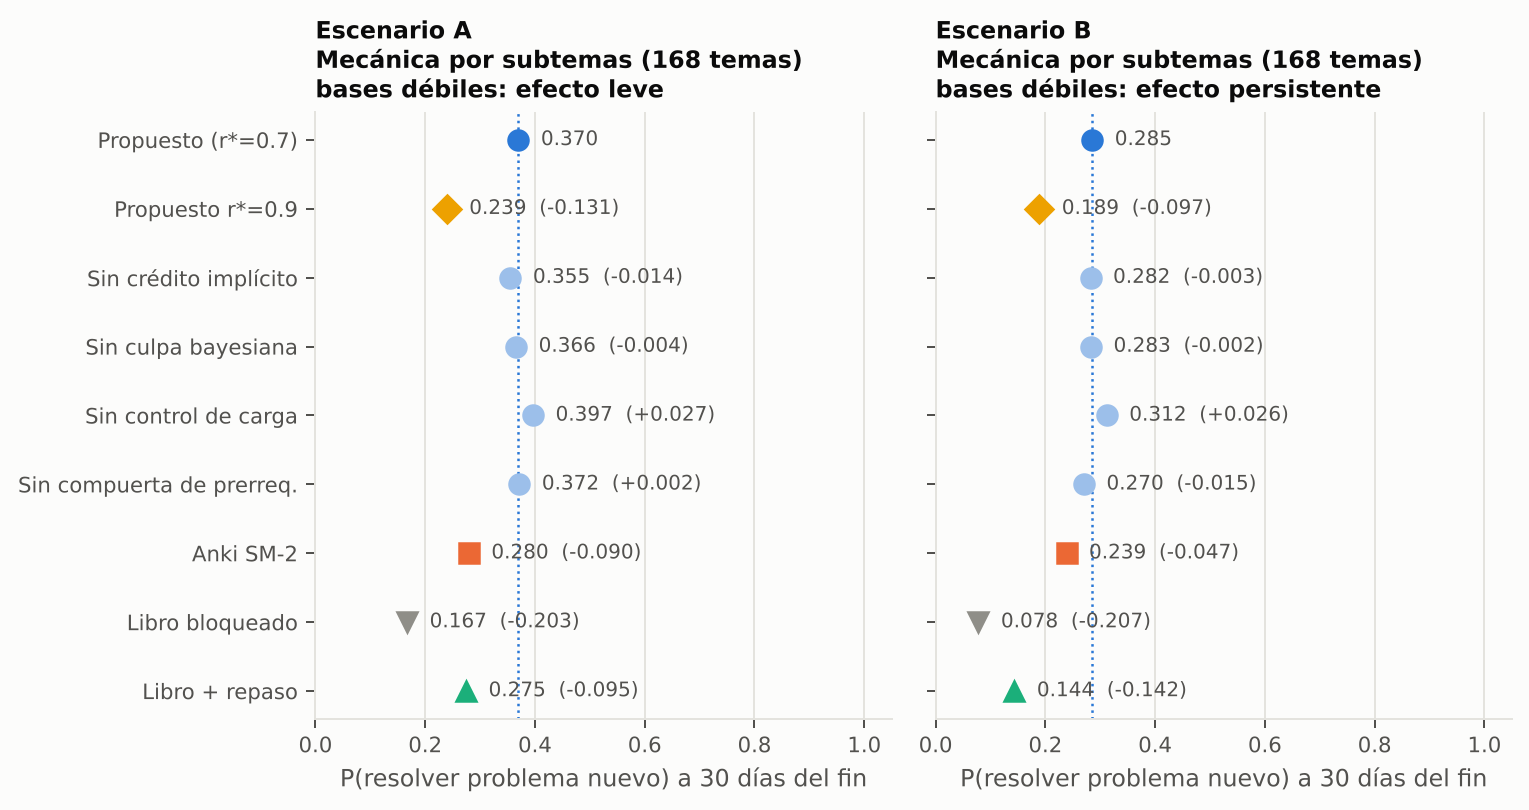
\includegraphics[width=0.84\textwidth]{figuras/subtemas_comparacion.png}

\footnotesize Propuesto frente a Anki: $\mathbf{+0.090}$ (A) y $\mathbf{+0.047}$ (B). Crédito implícito: $+0.014$ (A). Compuerta: $+0.015$ (B).
\end{frame}

%---------------------------------------------------------------
\begin{frame}{¿Por qué gana? Cobertura}
\centering
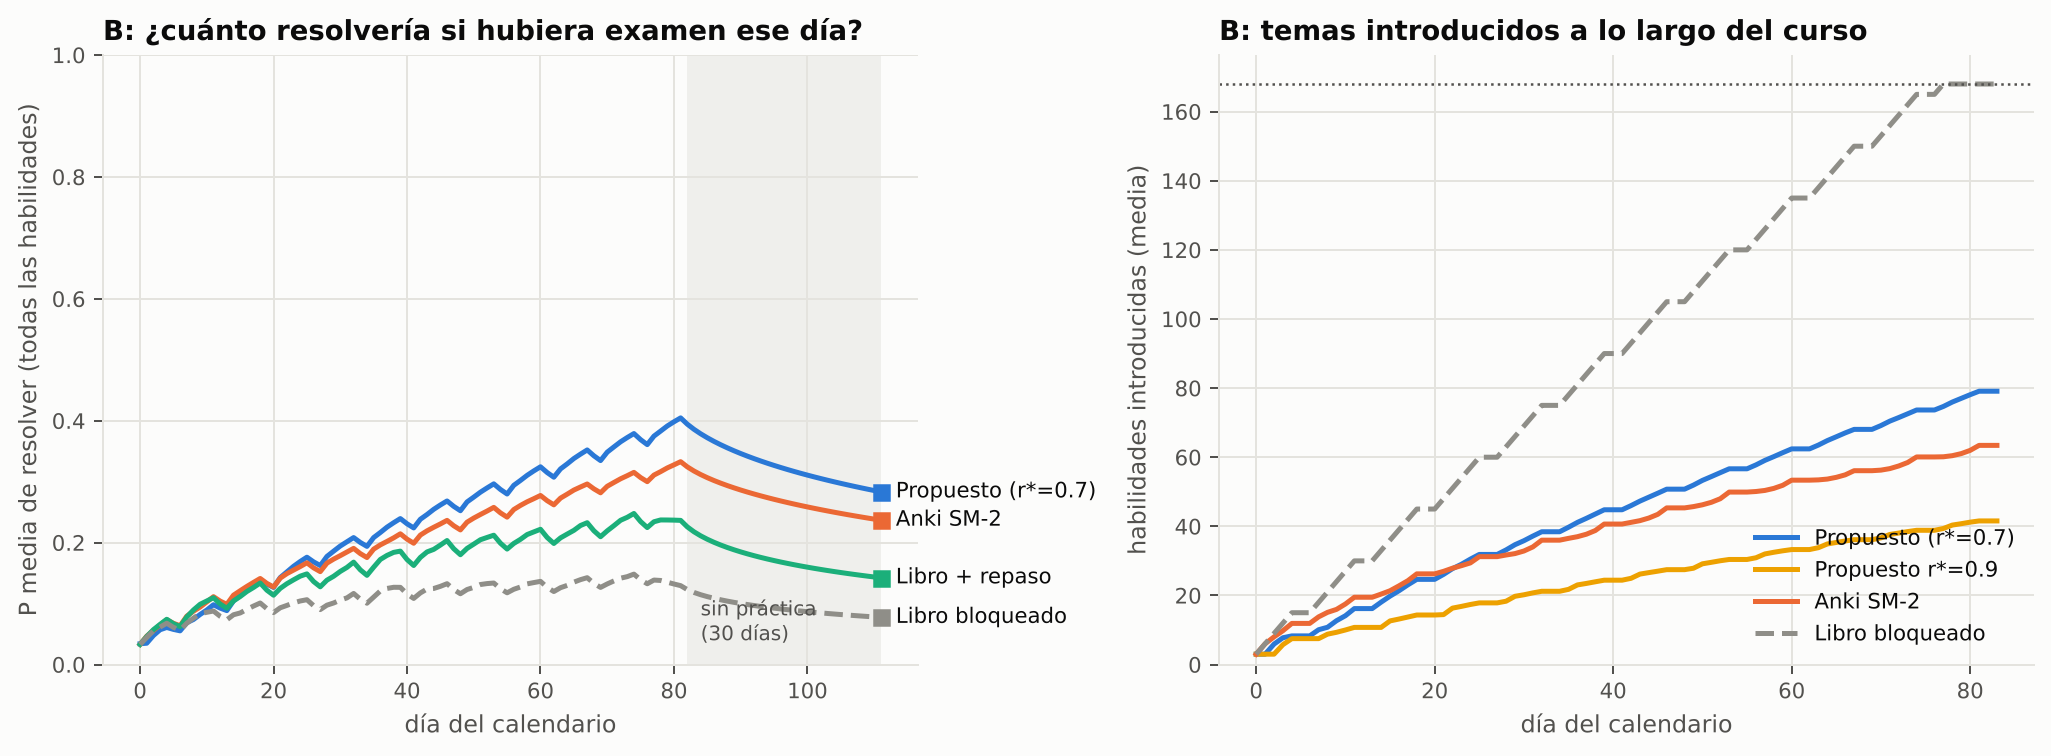
\includegraphics[width=0.88\textwidth]{figuras/subtemas_trayectorias.png}

\small Anki se atasca con sus repasos vencidos y deja de introducir temas (63 contra 79). Con $\rstar=0.9$, el propuesto repasa tan seguido que casi no avanza.
\end{frame}

%---------------------------------------------------------------
\begin{frame}{Pero ojo: cobertura frente a retención}
\begin{columns}[c]
\column{0.54\textwidth}
\small
\begin{tabular}{@{}lccc@{}}
\toprule
Escenario A & Temas & $P\ge0.8$ & $P$ en vistos \\
\midrule
Propuesto & 106 & 5.5 & $\approx0.58$ \\
Anki SM-2 & 71 & 11.0 & $\approx0.64$ \\
Propuesto $\rstar=0.9$ & 56 & 12.6 & $\approx0.68$ \\
\bottomrule
\end{tabular}
\column{0.43\textwidth}
\begin{itemize}\small
\item El propuesto gana porque \alert{cubre más temas}, con una retención algo menor por tema.
\item Si la meta es dominar pocos temas a fondo, la conclusión se invierte.
\item $\rstar$ no es un detalle técnico: es una \alert{decisión pedagógica} sobre esta frontera.
\end{itemize}
\end{columns}
\end{frame}

%---------------------------------------------------------------
\begin{frame}{La ventaja se mantiene con distintos presupuestos}
\centering
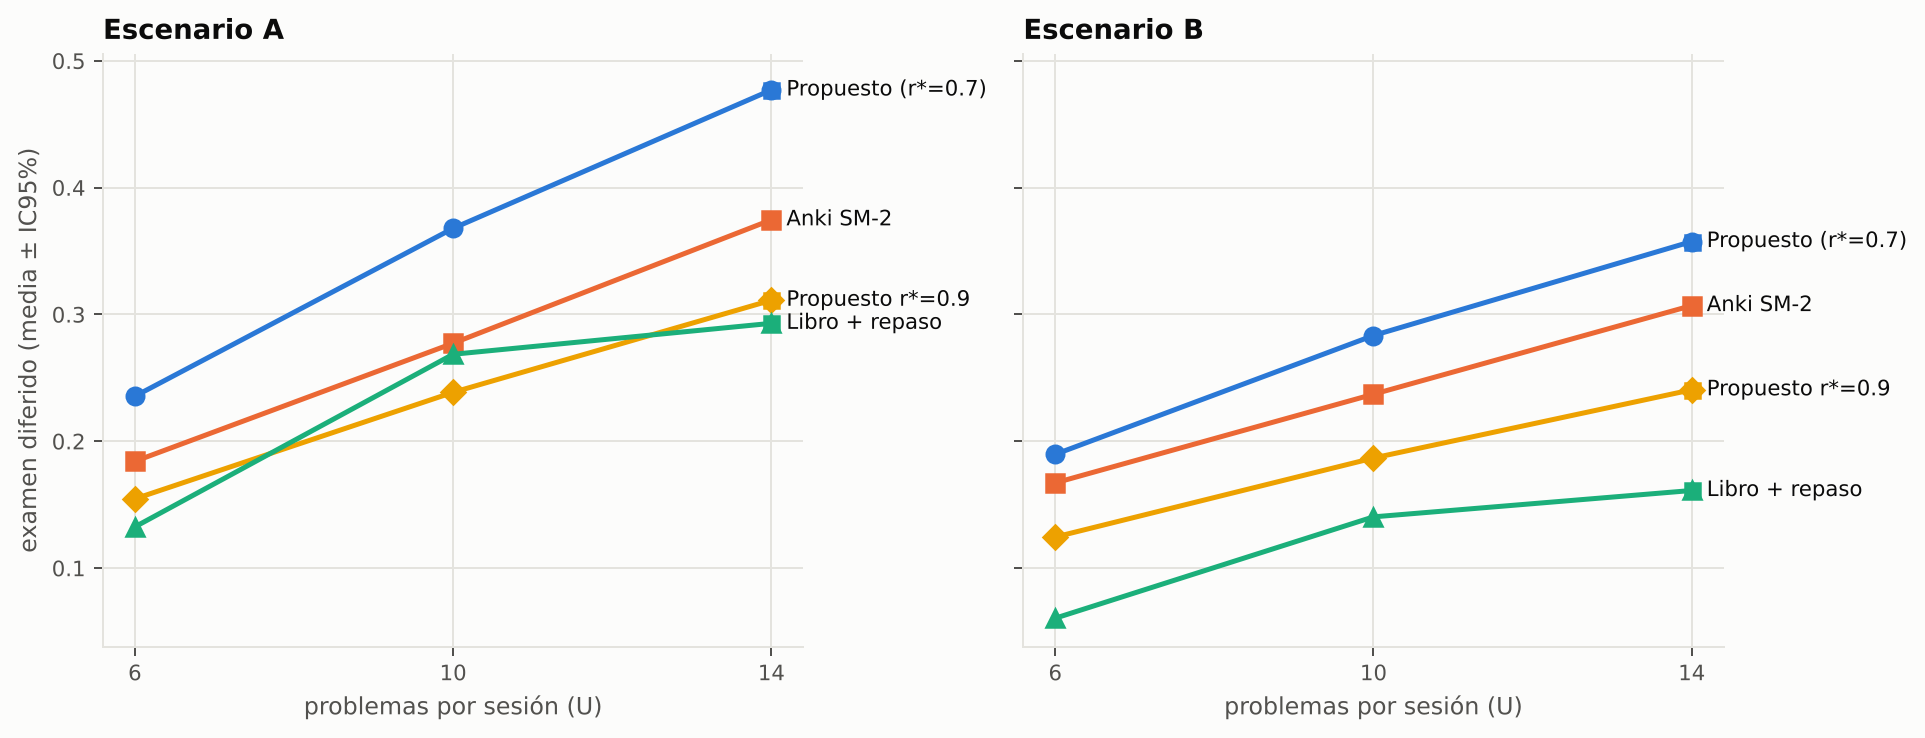
\includegraphics[width=0.88\textwidth]{figuras/subtemas_presupuesto.png}
\end{frame}

%---------------------------------------------------------------
\begin{frame}{La estructura del grafo importa}
\begin{columns}[c]
\column{0.5\textwidth}
\small
\begin{tabular}{@{}lcc@{}}
\toprule
Escenario B & Dependencias & Lineal \\
\midrule
Propuesto & 0.285 & \alert{0.124} \\
Anki SM-2 & 0.239 & 0.238 \\
Sin compuerta & 0.270 & 0.234 \\
Temas (propuesto) & 79 & 28 \\
\bottomrule
\end{tabular}
\column{0.48\textwidth}
\begin{itemize}\small
\item En cadenas lineales hay 103 niveles y sólo un tema admisible a la vez.
\item La compuerta serializa el curso y el propuesto se hunde; Anki ignora el grafo y no sufre.
\end{itemize}
\end{columns}
\vspace{5mm}
\begin{block}{Moraleja}
Un grafo con dependencias falsas castiga justo al sistema que lo respeta. \alert{La fidelidad del grafo importa tanto como la fórmula de repaso.}
\end{block}
\end{frame}

%---------------------------------------------------------------
\begin{frame}{Sensibilidad: retención objetivo y compuerta}
\centering
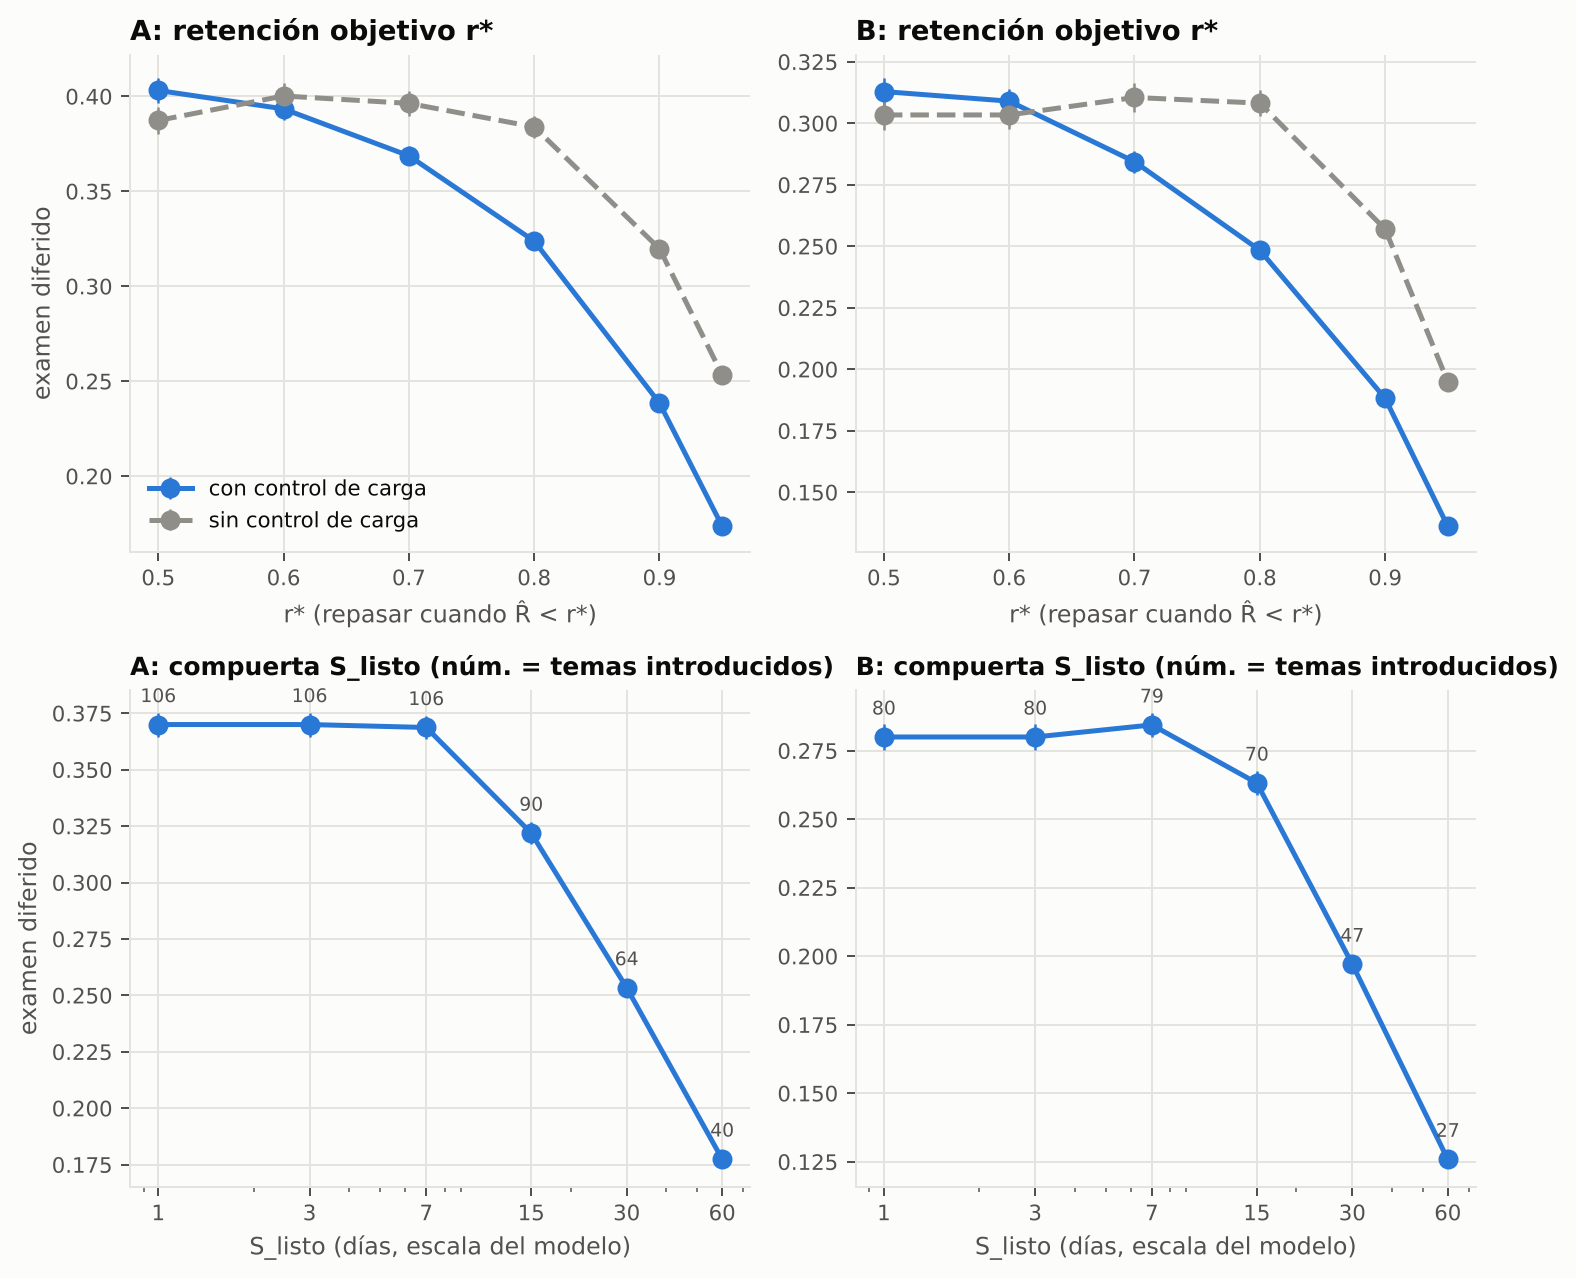
\includegraphics[height=0.74\textheight]{figuras/subtemas_sensibilidad.png}
\end{frame}

%---------------------------------------------------------------
\section{Discusión}

\begin{frame}{Limitaciones}
\begin{itemize}
\item \textbf{La verdad es un modelo}: dice qué \emph{podría} importar, no cuánto se gana en un aula.
\item \textbf{$\rstar=0.7$ se eligió después} de un barrido preliminar; hay que fijarlo sin usar la verdad.
\item \textbf{La métrica premia la cobertura}; un $\rstar$ bajo implica más fallos y posibles costos de motivación.
\item \textbf{Grafo de subtemas}: las 279 dependencias son un borrador sin validación docente.
\item \textbf{Simplificaciones}: culpa sin $s$ ni $g$, $\Sh_0$ común, sin efectos por alumno; $\hat\lambda\approx0$ en un escenario (identificabilidad).
\item \textbf{No se modela} intercalado, fatiga, ejemplos resueltos ni variación entre instancias.
\end{itemize}
\end{frame}

%---------------------------------------------------------------
\begin{frame}{Próximos pasos}
\begin{enumerate}
\item Culpa completa con $s$ y $g$; estimar $s$, $g$ y $w_{jk}$.
\item Validar el grafo de subtemas con docentes.
\item Piloto real $\rightarrow$ modelo jerárquico; comparar olvido exponencial y de potencia.
\item Criterio explícito para $\rstar$ (cobertura frente a dominio).
\item \textbf{Experimento}: intra-sujeto contrabalanceado (Lindsey et al.\ 2014), propuesto frente a FSRS/SM-2, tiempo igualado, prueba a 30 días.\\
{\small $n=7.85/d_z^2$: 32 alumnos para $d_z=0.5$; 88 para $d_z=0.3$.}
\end{enumerate}
\end{frame}

%---------------------------------------------------------------
\begin{frame}{Preguntas para discutir}
\begin{enumerate}
\item \textbf{Granularidad}: ¿subtemas, o habilidades todavía más finas?
\item \textbf{Objetivo pedagógico}: ¿maximizar cobertura o dominio? Eso fija $\rstar$.
\item \textbf{Validación del grafo}: ¿con qué docentes o con qué datos?
\item \textbf{Alcance de la tesis}: ¿modelo + simulación + piloto, o hasta el experimento en aula?
\item \textbf{Posicionamiento}: frente a Choffin et al.\ (2021) y Math Academy, ¿la contribución es el modelo formal, la evaluación o ambas?
\end{enumerate}
\end{frame}

%---------------------------------------------------------------
\appendix
\begin{frame}[standout]
Respaldo
\end{frame}

\begin{frame}{Respaldo: parámetros de la verdad simulada}
\small
\begin{columns}[T]
\column{0.5\textwidth}
\begin{tabular}{@{}lll@{}}
\toprule
& Valor & Significado \\
\midrule
$S_0$ & 0.6 d & estabilidad inicial \\
$\delta$ & 0.15 & penalización por profundidad \\
$a$ & $\ln4$ & escala de ganancia \\
$b$ & 0.15 & rendimientos decrecientes \\
$c$ & 2 & efecto de espaciamiento \\
\bottomrule
\end{tabular}
\column{0.5\textwidth}
\begin{tabular}{@{}lll@{}}
\toprule
& Valor & Significado \\
\midrule
$\ell$ & 0.6 & pérdida en un lapso \\
$\kappa$ & 4 d & consolidación de bases \\
$s,g$ & 0.05, 0.02 & descuido, adivinanza \\
$\sigma_\theta$ & 0.35 & heterogeneidad \\
$S_{\min}$ & 0.2 d & piso \\
\bottomrule
\end{tabular}
\end{columns}
\vspace{4mm}
Olvido: $R=(1+\tfrac{19}{81}\Delta t/S)^{-1/2}$, de modo que $R(S)=0.9$.
\end{frame}

\begin{frame}{Respaldo: calibración del modelo}
\centering
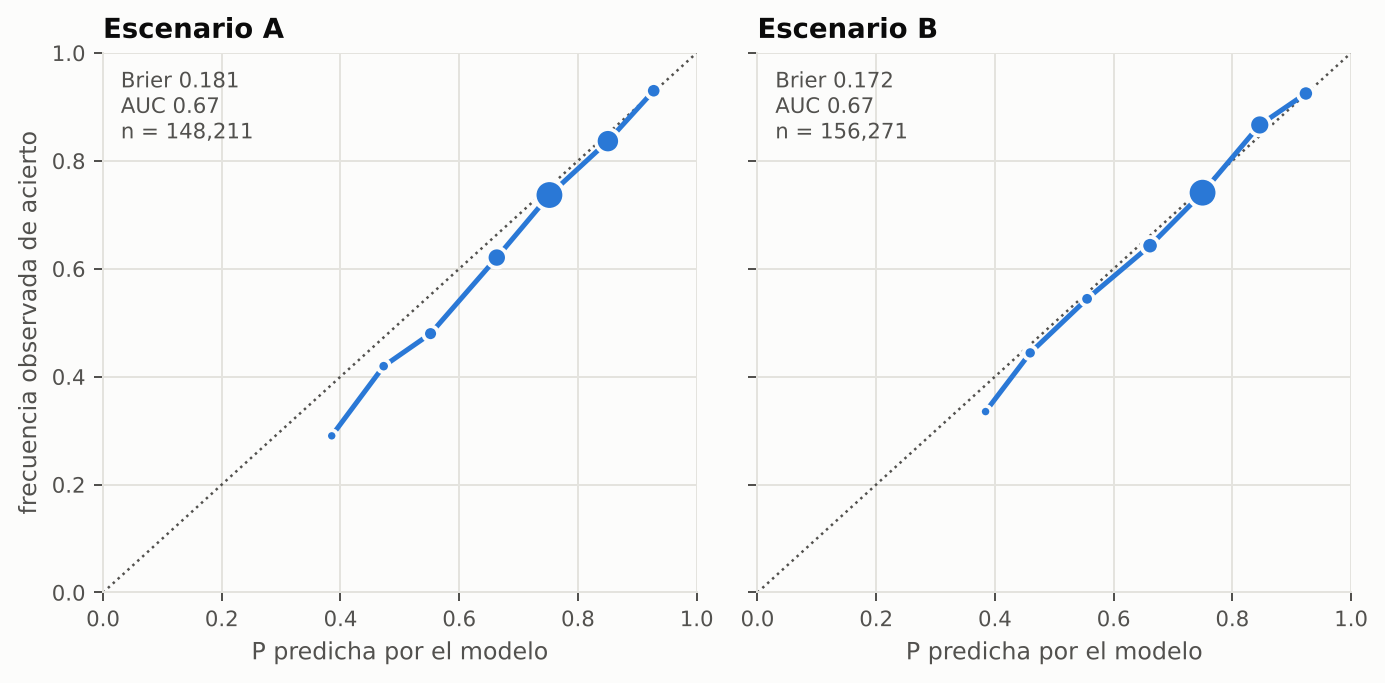
\includegraphics[width=0.8\textwidth]{figuras/subtemas_calibracion.png}

\small AUC $\approx0.67$. El modelo sobreestima en el rango medio, como era de esperar si la verdad olvida con ley de potencia.
\end{frame}

\end{document}
